\documentclass[author-year, review]{elsarticle} %review=doublespace preprint=single 5p=2 column
%%% Begin My package additions %%%%%%%%%%%%%%%%%%%
\usepackage[hyphens]{url}
\usepackage{lineno} % add 
%\linenumbers % turns line numbering on 
\bibliographystyle{elsarticle-harv}
\biboptions{sort&compress} % For natbib
\usepackage{graphicx}
\usepackage{booktabs} % book-quality tables
%% Redefines the elsarticle footer
\makeatletter
\def\ps@pprintTitle{%
 \let\@oddhead\@empty
 \let\@evenhead\@empty
 \def\@oddfoot{\it \hfill\today}%
 \let\@evenfoot\@oddfoot}
\makeatother

% A modified page layout
\textwidth 6.75in
\oddsidemargin -0.15in
\evensidemargin -0.15in
\textheight 9in
\topmargin -0.5in
%%%%%%%%%%%%%%%% end my additions to header



\usepackage[T1]{fontenc}
\usepackage{lmodern}
\usepackage{amssymb,amsmath}
\usepackage{ifxetex,ifluatex}
\usepackage{fixltx2e} % provides \textsubscript
% use upquote if available, for straight quotes in verbatim environments
\IfFileExists{upquote.sty}{\usepackage{upquote}}{}
\ifnum 0\ifxetex 1\fi\ifluatex 1\fi=0 % if pdftex
  \usepackage[utf8]{inputenc}
\else % if luatex or xelatex
  \usepackage{fontspec}
  \ifxetex
    \usepackage{xltxtra,xunicode}
  \fi
  \defaultfontfeatures{Mapping=tex-text,Scale=MatchLowercase}
  \newcommand{\euro}{€}
\fi
% use microtype if available
\IfFileExists{microtype.sty}{\usepackage{microtype}}{}
\usepackage{color}
\usepackage{fancyvrb}
\DefineShortVerb[commandchars=\\\{\}]{\|}
\DefineVerbatimEnvironment{Highlighting}{Verbatim}{commandchars=\\\{\}}
% Add ',fontsize=\small' for more characters per line
\newenvironment{Shaded}{}{}
\newcommand{\KeywordTok}[1]{\textcolor[rgb]{0.00,0.44,0.13}{\textbf{{#1}}}}
\newcommand{\DataTypeTok}[1]{\textcolor[rgb]{0.56,0.13,0.00}{{#1}}}
\newcommand{\DecValTok}[1]{\textcolor[rgb]{0.25,0.63,0.44}{{#1}}}
\newcommand{\BaseNTok}[1]{\textcolor[rgb]{0.25,0.63,0.44}{{#1}}}
\newcommand{\FloatTok}[1]{\textcolor[rgb]{0.25,0.63,0.44}{{#1}}}
\newcommand{\CharTok}[1]{\textcolor[rgb]{0.25,0.44,0.63}{{#1}}}
\newcommand{\StringTok}[1]{\textcolor[rgb]{0.25,0.44,0.63}{{#1}}}
\newcommand{\CommentTok}[1]{\textcolor[rgb]{0.38,0.63,0.69}{\textit{{#1}}}}
\newcommand{\OtherTok}[1]{\textcolor[rgb]{0.00,0.44,0.13}{{#1}}}
\newcommand{\AlertTok}[1]{\textcolor[rgb]{1.00,0.00,0.00}{\textbf{{#1}}}}
\newcommand{\FunctionTok}[1]{\textcolor[rgb]{0.02,0.16,0.49}{{#1}}}
\newcommand{\RegionMarkerTok}[1]{{#1}}
\newcommand{\ErrorTok}[1]{\textcolor[rgb]{1.00,0.00,0.00}{\textbf{{#1}}}}
\newcommand{\NormalTok}[1]{{#1}}
\usepackage{graphicx}
% We will generate all images so they have a width \maxwidth. This means
% that they will get their normal width if they fit onto the page, but
% are scaled down if they would overflow the margins.
\makeatletter
\def\maxwidth{\ifdim\Gin@nat@width>\linewidth\linewidth
\else\Gin@nat@width\fi}
\makeatother
\let\Oldincludegraphics\includegraphics
\renewcommand{\includegraphics}[1]{\Oldincludegraphics[width=\maxwidth]{#1}}
\ifxetex
  \usepackage[setpagesize=false, % page size defined by xetex
              unicode=false, % unicode breaks when used with xetex
              xetex]{hyperref}
\else
  \usepackage[unicode=true]{hyperref}
\fi
\hypersetup{breaklinks=true,
            bookmarks=true,
            pdfauthor={},
            pdftitle={Avoiding tipping points in the management of ecological systems: a non-parametric Bayesian approach},
            colorlinks=true,
            urlcolor=blue,
            linkcolor=magenta,
            pdfborder={0 0 0}}
\urlstyle{same}  % don't use monospace font for urls
\setlength{\parindent}{0pt}
\setlength{\parskip}{6pt plus 2pt minus 1pt}
\setlength{\emergencystretch}{3em}  % prevent overfull lines
\setcounter{secnumdepth}{0}
% Pandoc toggle for numbering sections (defaults to be off)
\setcounter{secnumdepth}{0}
% Pandoc header



\begin{document}
\begin{frontmatter}
  \title{Avoiding tipping points in the management of ecological systems: a
         non-parametric Bayesian approach}
  \author[cstar]{Carl Boettiger\corref{cor1}}
  \cortext[cor1]{Corresponding author}
  \ead{cboettig@ucsc.edu}
  \author[cstar]{Marc Mangel}
  \author[noaa]{Stephan B. Munch}
  \address[cstar]{Center for Stock Assessment Research, Department of Applied Math and Statistics, University of California, Mail Stop SOE-2, Santa Cruz, CA 95064, USA}
  \address[noaa]{Southwest Fisheries Science Center, National Oceanic and Atmospheric Administration, 110 Shaffer Road, Santa Cruz, CA 95060, USA}
 \end{frontmatter}


\section{Abstract}

Decision-theoretic methods often rely on simple parametric models of
ecological dynamics to compare the value of a potential sequence of
actions. Unfortunately, such simple models rarely capture the complexity
or uncertainty found in most real ecosystems. Non-parametric Bayesian
methods offer a promising statistical approach for predictive modeling
of ecological dynamics in regions of state space where the data is
adequate, while at the same time offering more flexible patterns with
greater uncertainty outside the observed data. This contrasts from
simple parametric models which provide relatively constant level of
uncertainty in regions with and without adequate data. The consequence
of such misplaced confidence outside the data can lead to highly
undesirable results that may be avoided with the more flexible
non-parametric Bayesian approach.

\section{Introduction}

Most management recommendations from the ecological literature are based
on (or at least motivated by) parametric models. Though in principle
these models reflect mechanistic underpinnings of biological
interactions involved, in practice real mechanisms are often unknown and
the true dynamics too complex to be captured by simple models. While
simple mechanistic models can nevertheless provide important insights
into possible dynamics -- for instance, demonstrating that a vaccine
does not have to be 100\% effective to eliminate the transmission of a
virus -- such approaches are not well-suited for use in forecasting
outcomes of potential management options. Non-parametric approaches
offer a more flexible alternative that can both more accurately reflect
the data available while also representing greater uncertainty in areas
(of state-space) where data is lacking. Ecological research and
management strategy should pay closer attention to the opportunities and
challenges nonparametric modeling can offer.

\subsubsection{Quantitative vs Qualitative Decisions}

In this paper, we consider those ecological management problems in which
a mathematical (or computational) model is used to quantitatively inform
decision-making by allowing a manager to compare to the expected
consequences of potential management actions (or policies). We
distinguish this from the solely qualitative use of a model, in which
models are used to represent and compare hypotheses of different
mechanisms that would lead to qualitatively different actions.

Though simple mechanistically motivated models may be best for the
latter case (Cuddington, Fortin, and Gerber 2013; Geritz and Kisdi
2012), such models can be not only inaccurate but misleading in
quantitative decision making. This arises for two reasons:

\begin{enumerate}
\def\labelenumi{\arabic{enumi}.}
\itemsep1pt\parskip0pt\parsep0pt
\item
  We do not know what the correct parameter values are for the models.
\item
  We do not know what the correct models are for ecological systems.
\end{enumerate}

The complexity of ecological interactions and a lack of data contribute
greatly to both of the problems. This concern is particularly acute in
case of ecological tipping points (Barnosky et al. 2012; Scheffer et al.
2001), which arise from feedbacks common in ecological systems and can
lead to a sudden catastrophic transition to an undesirable state. In
general we do not know where such tipping points are unless we have
already observed the transition, in which case it is frequently too late
to respond. Though there may exist early warning signals for certain
kinds of these transitions that are driven by slow changes (Scheffer et
al. 2009), we do not know when, where, or how to apply them to the
decision making context more generally (Boettiger and Hastings 2013).

In addition to facing the potentially grave consequences of such
transitions, if they do exist in a system of interest, this generally
means that we lack data in the region near and beyond a possible tipping
point. As a consequence, our models are least accurate just where we
need them to be most accurate.\\Unfortunately, parametric modeling
approaches are not well-suited to this scenario, in which good data is
avialble over only part of the relevant state-space. Necessary
assumptions about model structure in any parametric approach can lead
such models to perform very poorly, even when accounting for parameter
uncertainty.

Non-parametric models can more realistically represent uncertainties
outside of observed data while also better capturing the dynamics in the
region observed. Advances in the theory and computational
implementations of nonparametric methods make them ripe for such
applications. We use the classic problem of optimal harvest of a marine
fishery to illustrate how the nonparametric approach of Gaussian
processes can be applied. We will compare Bayesian implementations of
both nonparametric and parametric models, which best allow us to capture
the uncertainty of model estimation in either case and permits a more
natural comparison between approaches.

\subsubsection{Terminology: ``Non-parametric''}

The term non-parametric to describe modeling approaches such as Gaussian
processes is a common source of confusion, notwithstanding the fact that
the model is still specified by parameters. Some literature has
introduced the term ``semi-parametric'' in tacit acknowledgment of this,
which no doubt only contributes to the confusion. The problem is further
exacerbated by the several meanings assigned to the term in statistics:
(a) that the method does not assume some particular probability
distribution (e.g.~a non-parametric bootstrap) or (b) that the method
does not assume a fixed structure to the model. Our use is that of (b),
in contrast to the classical approaches that do. The difference is
clearest by way of example.

\subsubsection{Uncertainties: the classical approach}

The ecological dynamics of most systems of management interest are
typically both complex and unknown. Despite this, quantitative policy
optimization in these systems has almost exclusively been based on
simple, mechanistically motivated parametric models. There are several
reasons for this. First, limited available data almost always precludes
any accurate estimate of more complicated models. Second, the
computational demands of determining an optimal strategy in a sequential
decision-theory problem suffer from the ``curse of dimensionality'' that
makes it difficult to consider more complicated models, states, or
actions. Unfortunately, these challenges also make it particularly
difficult to reflect the true uncertainty either in the parameters of
the given models (parametric uncertainty) or in the structure of the
models themselves (structural uncertainty). Further unknowns such as
measurement uncertainty, parameter uncertainty, unobserved states,
knowledge of boundary conditions, etc. further compound the issue.
Though a hierarchical Bayesian approach provides a natural way to
address these from a statistical standpoint, formulating reasonable
parametric descriptions of each form of uncertainty is a challenging
task in itself, let alone the computational difficulties of solving such
a system. Cressie et al. (2009) provides a good account of the successes
and challenges of the approach. Applying these approaches in the
management context of sequential decision making, in which forecasts
must be obtained over a range of possible actions and updated regularly
as new information arrives makes such an approach less feasible still.

An active literature and growing computational power over the past
several decades have only marginally improved this situation. Parametric
or structural uncertainty can be introduced only by increasing the state
space to reflect a distribution of possible parameters or the degree of
belief in each of a set of possible models Frequently, the space of
possible actions must then be reduced or the algorithms adjusted by
approximations to keep computations feasible.

Traditional approaches to optimal control (Pontryagin's principle,
stochastic dynamic programming) rely on knowledge of the state equation,
usually described by a simple parametric model. Here we illustrate how a
stochastic dynamic programming algorithm can alternatively be driven by
the predictions from a Gaussian process.

\section{Approach and Methods}

\subsection{Underlying Model}

Concerns over the potential for tipping points in ecological dynamics
(Scheffer et al. 2001) highlight the dangers of uncertainty in
ecological management and pose a substantial challenge to existing
decision-theoretic approaches (Brozović and Schlenker 2011). Because
intervention is often too late after a tipping point has been crossed
(but see Hughes et al. (2013)), management is most often concerned with
avoiding potentially catastrophic tipping points before any data is
available at or following a transition that would more clearly reveal
these regime shift dynamics (e.g. Bestelmeyer et al. 2012).

To illustrate the value of the non-parametric Bayesian approach to
management, we focus on example of a system containing such a tipping
point whose dynamics can still be described by a simple, one-dimensional
parametric model.\\We will focus on a simple parametric model for a
single species (derived from fist principles by Allen et al. 2005) as
our underlying ``reality''.

\begin{align}
X_{t+1} &= Z_t f(S_t) \\
S_t &= X_t - h_t \\
f(S_t) &= e^{r \left(1 - \frac{S_t}{K}\right)\left(S_t - C\right)}
\end{align}

Where $Z_t$ is multiplicative noise function with mean 1, representing
stochastic growth. We will consider log-normal noise with shape
parameter $\sigma_g$. We start with an example in which the parameters
are $r =2$, $K=8$, $C=5$ and $\sigma_g = 0.1$.

As a low-dimensional system completely described by three parameters,
this scenario should if anything be favorable to a parametric-based
approach. This model contains an Allee effect, or tipping point, below
which the population is not self-sustaining and shrinks to zero
(Courchamp, Berec, and Gascoigne 2008).

Both parametric and nonparametric approaches will require training data
on which to base their model of the process. We generate the training
data under the model described in Eq 1 for $T_{\textrm{obs}}=40$ time
steps, under a known but not necessarily optimal sequence of harvest
intensities, $h_t$. For simplicity we imagine a fishery that started
from zero harvest pressure and has been gradually increasing the
harvest.

\textbf{\emph{Should we include any emprical examples?}}

\subsubsection{The optimal control problem in fisheries management}

In our example, we focus on the problem in which a manager must set the
harvest level for a marine fishery each year to maximize the net present
value of the resource, given an estimated stock size from the year
before. Rich data and global concerns have made marine fisheries the
crucible for much of the founding work (Gordon 1954; Reed 1979; May et
al. 1979; Ludwig and Walters 1982) in managing ecosystems under
uncertainty. Global trends (Worm et al. 2006) and controversy (Hilborn
2007; Worm et al. 2009) have made understanding these challenges all the
more pressing.

To permit comparisons against a theoretical optimum we will consider
data on the stock dynamics simulated from a simple parametric model in
which recruitment of the fish stock $X_{t+1}$ in the following year is a
stochastic process governed by a function $f$ of the current stock
$X_t$, selected harvest policy $h_t$, and noise process $Z$,

\[X_{t+1} = Z_t f(X_t, h_t) \]

Given parameters for the function $f$ and probability distribution $Z$,
along with a given economic model determining the price/profit
$\Pi(X_t, h_t)$ realized in a given year given a choice of harvest $h_t$
and observed stock $X_t$. This problem can be solved exactly for
discretized values of stock $X$ and policy $h$ using stochastic dynamic
programming (SDP) (Mangel 1985). Problems of this sort underpin much
marine fisheries management today.

A crux of this approach is correctly specifying the functional form of
$f$, along with its parameters. The standard approach uses one of a
handful of common parametric models representing the stock-recruitment
relationship, usually after estimating the model parameters from any
available existing data. Uncertainty in the parameter estimates can be
estimated and integrated over to determine the optimal policy under
under uncertainty (Mangel 1985; Schapaugh and Tyre 2013). Uncertainty in
the model structure itself can only be addressed in this approach by
hypothesizing alternative model structures, and then performing some
model choice or model averaging (B. K. Williams 2001; Athanassoglou and
Xepapadeas 2012). For simplicity of the comparison we consider only the
case of a structurally correct and structurally incorrect model, and
estimate Bayesian posterior distributions of the parameters. We will
also compare to a simpler maximum likelihood estimate of the parameters
that ignores the issue of parameter uncertainty.

We compare these parametric approaches to our alternative that uses a
Gaussian Process (GP) in place of a given stock recruitment curve. We
briefly revisit a description of the Gaussian Process approach that has
appeared in recent literature before describing how we take the
important step of adapting the GP to the decision theory problem that
can still be solved using SDP.

\subsubsection{The Non-parametric Bayesian alternative for
stock-recruitment curves}

The use of Gaussian process (GP) regression (or ``kreging'' in the
geospatial literature) to formulate a predictive model is relatively new
in the context of modeling dynamical systems (Kocijan et al. 2005) and
introduced in the ecological modeling and fisheries management by Munch
et al. (2005). An accessible and thorough introduction to the
formulation and use of GPs can be found in Rasmussen and Williams
(2006).

The essence of the GP approach can be captured in the following thought
experiment: An exhaustive parametric approach to the challenge of
structural uncertainty might proceed by writing down all possible
functional forms for the underlying dynamical system with all possible
parameter values for each form, and then consider searching over this
huge space to select the most likely model and parameters; or using a
Bayesian approach, assign priors to each of these possible models and
infer the posterior distribution of possible models. The GP approach can
be thought of as a computationally efficient approximation to this
approach. GPs represent a large class of models that can be though of as
capturing or reasonably approximating the set of models in this
collection. By modeling at the level of the process, rather than the
level of parametric equation, we can more concisely capture the possible
behavior of these curves. In place of a parametric model of the
dynamical system, the GP approach postulates a prior distribution of
(n-dimensional) curves that can be though of as approximations to a
range of possible (parametric) models that might describe the data. The
GP allows us to consider a set of possible curves simultaneously.

\subsubsection{Background on Gaussian Process inference}

Once the posterior Gaussian process (GP) has been estimated (e.g.~see
Munch et al. 2005), it is necessary to adapt it in place of the
parametric equation for the stochastic dynamic programming (SDP)
solution (see Mangel and Clark 1988 for a detailed description of
parametric SDP methods) to the optimal policy. The essence of the idea
is straight forward -- we will use the estimated GP in place of the
parametric growth function to determine the stochastic transition matrix
on which the SDP calculations are based. The SDP is solved in a
discretized state space -- both the continuously valued population
densities $X$ and harvest quotas $h$ are first mapped to a bounded,
discrete grid. (For simplicity we will consider a uniform grid, though
for either parametric or GP-based SDP it is often advantageous to use a
non-uniform discretization such as a basis function representation,
e.g.~see (Deisenroth, Rasmussen, and Peters 2009)).

The SDP approach then computes a transition matrix, $\mathbf{F}$. We
demonstrate that calculation is just as straight forward based on the GP
as it is in the classical context using the parametric model. The
${i,j}$ of the transition matrix $F$ entry gives the probability of
transitioning into state $x_i$ given that the system is in state $x_j$
in the previous time-step. To generate the transition matrix based on
the posterior GP, we need only the expected values at each grid point
and the corresponding variances (the diagonal of the covariance matrix),
as shown in Figure 1. Given the mean of the GP posterior at each
grid-point as the vector $E$ and variance at that point as vector $V$,
the probability of transitioning from state $x_i$ to state $x_j$ is

\[\mathcal{N}\left(x_j \vert  \mu = E_i, \sigma = \sqrt{V_i}\right)\]

where $\mathcal{N}$ is the Normal density at $x_j$ with mean $\mu$ and
variance $\sigma^2$. Strictly speaking, the transition probability
should be calculated by integrating the normal density over the bin of
width $\Delta$ centered at $x_j$. For a sufficiently fine grid that
$f(x_j) \approx f(x_j + \Delta)$, it is sufficient to calculate the
density at $x_j$ and then row-normalize the transition matrix. The
process can then be repeated for each possible discrete value of our
control variable, (harvest $h$).

\textbf{Pseudocode for the determining the transition matrix from the
GP}

\begin{Shaded}
\begin{Highlighting}[]
\NormalTok{for(h in h_grid)}
  \NormalTok{F_h = for(x_j in grid)}
          \NormalTok{for(i in }\DecValTok{1}\NormalTok{:N) }
            \KeywordTok{dnorm}\NormalTok{(x_j, mu[i]-h, V[i])}
\end{Highlighting}
\end{Shaded}

Using the discrete transition matrix we may write down the Bellman
recursion defining the stochastic dynamic programming iteration:

\begin{equation}
V_t(x_t) = \max_h \mathbf{E} \left( h_t + \delta V_{t+1}( Z_{t+1} f(x_t - h_t)) \right)
\end{equation}

where $V(x_t)$ is the value of being at state $x$ at time $t$, $h$ is
control (harvest level) chosen. Numerically, the maximization is
accomplished as follows. Consider the set of possible control values to
be the discrete values corresponding the grid of stock sizes. Then for
each $h_t$ there is a corresponding transition matrix $\mathbf{F}_h$
determined as described above but with mean $\mu = x_j - h_t$. Let
$\vec{V_t}$ be the vector whose $i$th element corresponds to the value
of having stock $x_i$ at time $t$. Then let $\Pi_h$ be the vector whose
$i$th element indicates the profit from harvesting at intensity $h_t$
given a population $x_i$ (e.g. $\max(x_i, h_t)$ since one cannot harvest
more fish then the current population size). Then the Bellman recursion
can be given in matrix form as

\[V_{t} = \max_h \left( \Pi_{h_{t}} + \delta \mathbf{F}_h V_{t+1} \right)\]

where the sum is element by element and the expectation is computed by
the matrix multiplication $\mathbf{F} V_{t+1}$.

\subsubsection{Pseudocode for the Bellman iteration}

\begin{Shaded}
\begin{Highlighting}[]
 \NormalTok{V1 <- }\KeywordTok{sapply}\NormalTok{(}\DecValTok{1}\NormalTok{:}\KeywordTok{length}\NormalTok{(h_grid), function(h)\{}
      \NormalTok{delta * F[[h]] %*% V +  }\KeywordTok{profit}\NormalTok{(x_grid, h_grid[h]) }
    \NormalTok{\})}
    \CommentTok{# find havest, h that gives the maximum value}
    \NormalTok{out <- }\KeywordTok{sapply}\NormalTok{(}\DecValTok{1}\NormalTok{:gridsize, function(j)\{}
      \NormalTok{value <- }\KeywordTok{max}\NormalTok{(V1[j,], }\DataTypeTok{na.rm =} \NormalTok{T) }\CommentTok{# each col is a diff h, max over these}
      \NormalTok{index <- }\KeywordTok{which.max}\NormalTok{(V1[j,])  }\CommentTok{# store index so we can recover h's }
      \KeywordTok{c}\NormalTok{(value, index) }\CommentTok{# returns both profit value & index of optimal h.  }
    \NormalTok{\})}
    \CommentTok{# Sets V[t+1] = max_h V[t] at each possible state value, x}
    \NormalTok{V <- out[}\DecValTok{1}\NormalTok{,]                        }\CommentTok{# The new value-to-go}
    \NormalTok{D[,OptTime-time}\DecValTok{+1}\NormalTok{] <- out[}\DecValTok{2}\NormalTok{,]       }\CommentTok{# The index positions}
\end{Highlighting}
\end{Shaded}

This completes the algorithm adapting the GP to the sequential
decision-making problem through SDP, which we believe has not yet been
demonstrated in the literature. We provide an R package implementation
of this, along with the Gaussian process inference, in the supplemental
materials.

\subsubsection{Estimating parametric models}

We estimate posterior distributions for two parametric models: one using
the structurally correct model as given in Eq (1), which we refer to as
the ``Parametric Bayes'' model, and another using the familiar Ricker
model, using a Gibbs sampler as described (with source code) in the
appendix). In addition we estimate the parameters of the structurally
correct model by maximum likelihood.

The posterior distribution for the hyper-parameters of the Gaussian
process model are estimated by Metropolis-Hastings algorithm, again with
details and code provided in the Appendix. Rasmussen and Williams (2006)
provides an excellent general introduction to Gaussian Processes and
Munch et al. (2005) first discusses their application in this context.

\section{Results}

\begin{figure}[htbp]
\centering
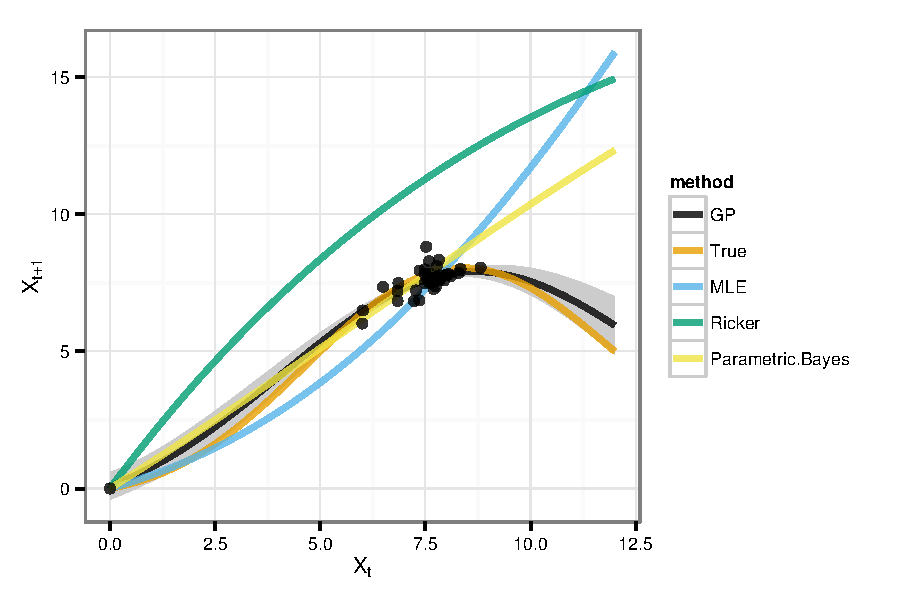
\includegraphics{Figure1.pdf}
\caption{Mean dynamics predicted by each model.}
\end{figure}

Figure 1 shows the mean inferred state space dynamics of each model
relative to the true model used to generate the data, predicting the
relationship between observed stock size (x-axis) to the stock size
after recruitment the following year. All models except the MLE model
estimate a distribution around the means shown here, and all models
estimate a level of process noise, which is independent of the state
value (x). Note that in contrast to the other models shown, the mean
Gaussian process corresponds to a distribution of curves - as indicated
by the gray band - which itself has a mean shown in black. Note that
this mean GP is thus more certain of the dynamics in the region where
data is available then where it is not.

While it would be natural (and straight forward) to condition the GP on
passing through the origin (0,0) (see appendix), the estimate shown here
is based only on the observed data. The observed data from which each
model is estimated is also shown. The observations come from only a
limited region of state space corresponding to unharvested or weakly
harvested system. No observations occur at the theoretical optimum or
near the tipping point.

\begin{figure}[htbp]
\centering
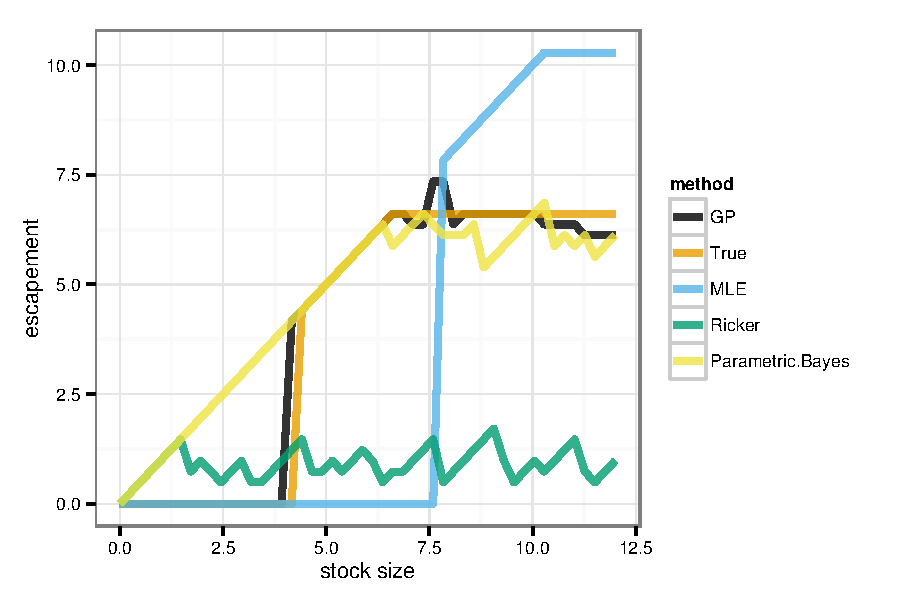
\includegraphics{Figure2.pdf}
\caption{Steady-state optimal policies by each model.}
\end{figure}

The resulting optimal management strategy based on each of the inferred
models is shown in Figure 2, against the optimal strategy given the true
underlying dynamics. Policies are shown in terms of target escapement,
$S_t$. Under models such as this a constant escapement policy is
expected to be optimal (Reed 1979), whereby population levels below a
certain size $S$ are unharvested, while above that size the harvest
strategy aims to return the population to $S$, resulting in the
hockey-stick shaped policies shown.

\begin{figure}[htbp]
\centering
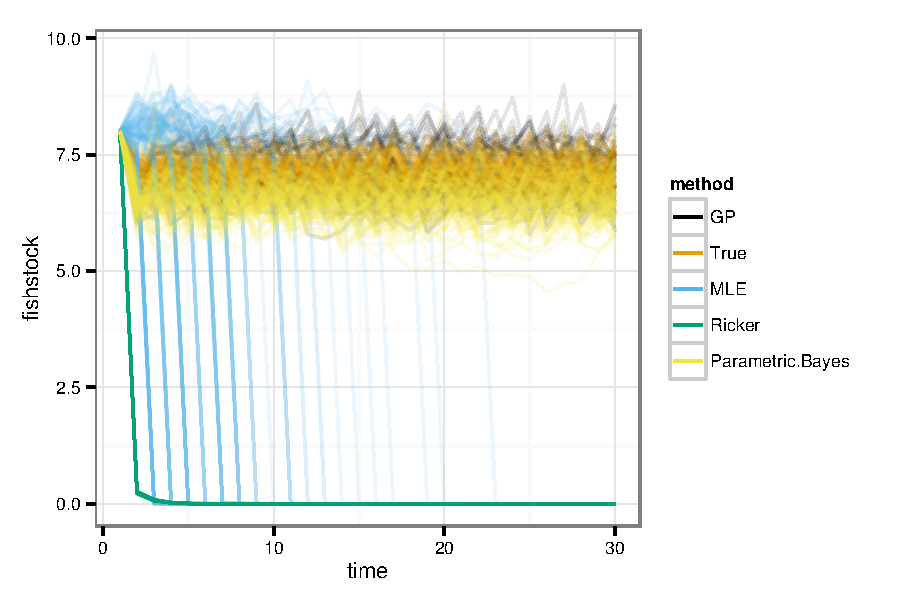
\includegraphics{Figure3.pdf}
\caption{Managing the simulated system over 100 replicate instances
under each policy}
\end{figure}

The consequences of managing 100 replicate realizations of the simulated
fishery under each of the policies estimated is shown in Figure 3. As
expected from the policy curves, the structurally correct model
under-harvests, leaving the stock to vary around it's un-fished optimum.
The structurally incorrect Ricker model over-harvests the population
passed the tipping point consistently, resulting in the immediate crash
of the stock and thus derives minimal profits.

The results shown in Figures 1-3 are not unique to the simulated data or
models chosen here, but arises across a range of parameter values and
simulations as shown in the supplemental figures. The results across
this range can most easily be compared by the relative differences in
net present value realized by each of the approaches, as shown in Figure
4. The Gaussian Process most consistently realizes a value close to the
optimal solution, and importantly avoids ever driving the system across
the tipping point, which results in the near-zero value cases in the
parametric models.

\begin{figure}[htbp]
\centering
\includegraphics{figure/figure4.png}
\caption{Histograms of the realized net present value of the fishery
over a range of simulated data and resulting parameter estimates. For
each data set, the three models are estimated as described above. Values
plotted are the averages of a given policy over 100 replicate
simulations. Details and code provided in the supplement.}
\end{figure}

\section{Discussion}

Non-parametric Bayesian methods have received far too little attention
in ecological modeling efforts that are aimed at improved conservation
planning and decision making support. Such approaches may be
particularly useful when the available data is restricted to a limited
area of state-space, which can lead parametric models to underestimate
the uncertainty in dynamics at population levels (states) which have not
been observed. One reason for the relative absence of nonparametric
approaches in the natural resource management context may be the lack of
existing approaches for adapting the non-parametric Bayesian models
previously proposed (Munch et al. 2005) to a decision-theoretic
framework. Adapting a non-parametric approach requires modification of
existing methods for decision theory. We have illustrated how this might
be done for a classic stochastic dynamic programming problem, opening
the door for substantial further research into how these applications
might be improved.

While non-parametric Bayesian approaches will not always be preferable
to simple mechanistic models, we highlight three aspects of the problem
consider here that make these methods particularly valuable. These
aspects are common to many conservation decision making problems, which
thus merit greater use of non-parametric approaches that can best take
advantage of them.

\subsubsection{1. Large uncertainty where the data is poor}

The parametric models perform worst when they propose a management
strategy outside the range of the observed data. The non-parametric
Bayesian approach, in contrast, allows a predictive model that expresses
a great deal of uncertainty about the probable dynamics outside the
observed range, while retaining very good predictive accuracy in the
range observed. The management policy dictated by the GP balance this
uncertainty against the immediate value of the harvest, and act to
stabilize the population dynamics in a region of state space in which
the predictions can be reliably reflected by the data.

\subsubsection{2. Predictive accuracy where data is good}

While expressing larger uncertainty outside the observed data, the GP
can also provide a better fit with smaller uncertainty inside the range
of the observed data. This arises from the greater flexibility of the
Gaussian process, which describes a large family of possible
curves.\\While in a parametric context this over-fitting would be more
worrisome -- a high-degree polynomial could fit the data even better --
those concerns are driven by the resulting parametric fit outside the
data, which may involve wild oscillations unsupported by the data. As we
have seen in \#1, the GP is less vulnerable to such unjustified
predictions outside the data, and is meanwhile free to benefit from the
greater fit where the data is available.

\subsection{Future directions}

In this simulated example, the underlying dynamics are truly governed by
a simple parametric model, allowing the parametric approaches to be more
accurate. Similarly, because the dynamics are one-dimensional dynamics
and lead to stable nodes (rather than other attractors such as
limit-cycles resulting in oscillations), the training data provides
relatively limited information about the dynamics. For these reasons, we
anticipate that in higher-dimensional examples characteristic of
ecosystem management problems that the machine learning approach will
prove even more valuable.

 Data complexity. Perhaps too far out of scope\ldots{} The nonparametric
Bayesian approach is also better suited to complex and disparate data.
Incorporating various sources of information into mechanistic models can
be an immensely difficult due to the increased complexity involved.

\subsubsection{Online learning}

In our treatment here we have ignored the possibility of learning during
the management phase, in which the additional observations of the stock
size could potentially improve parameter estimates. While we intend to
address this possibility in future work in the context of these
non-parametric models, we have not addressed it here for pedagogical
reasons. In the context presented here, it is clear that the differences
in performance arise from differences in the uncertainty inherent in the
model formulations, rather than from differing abilities to learn.
Because we consider a threshold system, online learning would not change
this generic feature of a lack of data in a certain range of the state
space which is better captured by the Gaussian process.

\section{Acknowledgments}

This work was partially supported by the Center for Stock Assessment
Research, a partnership between the University of California Santa Cruz
and the Fisheries Ecology Division, Southwest Fisheries Science Center,
Santa Cruz, CA and by NSF~grant EF-0924195 to MM.

\section{References}

Allen, Linda J. S., Jesse F. Fagan, Göran Högnäs, and Henrik Fagerholm.
2005. ``Population extinction in discrete-time stochastic population
models with an Allee effect.'' \emph{Journal of Difference Equations and
Applications} 11 (4-5) (apr): 273--293.
doi:10.1080/10236190412331335373.
\url{http://www.tandfonline.com/doi/abs/10.1080/10236190412331335373}.

Athanassoglou, Stergios, and Anastasios Xepapadeas. 2012. ``Pollution
control with uncertain stock dynamics: When, and how, to be
precautious.'' \emph{Journal of Environmental Economics and Management}
63 (3) (may): 304--320. doi:10.1016/j.jeem.2011.11.001.
\url{http://linkinghub.elsevier.com/retrieve/pii/S0095069611001409}.

Barnosky, Anthony D., Elizabeth a Hadly, Jordi Bascompte, Eric L.
Berlow, James H. Brown, Mikael Fortelius, Wayne M. Getz, et al. 2012.
``Approaching a state shift in Earth's biosphere.'' \emph{Nature} 486
(7401) (jun): 52--58. doi:10.1038/nature11018.
\url{http://www.nature.com/doifinder/10.1038/nature11018}.

Bestelmeyer, Brandon T., Michael C. Duniway, Darren K. James, Laura M.
Burkett, and Kris M. Havstad. 2012. ``A test of critical thresholds and
their indicators in a desertification-prone ecosystem: more resilience
than we thought.'' Ed. Katharine Suding. \emph{Ecology Letters} (dec).
doi:10.1111/ele.12045. \url{http://doi.wiley.com/10.1111/ele.12045}.

Boettiger, Carl, and Alan Hastings. 2013. ``Tipping points: From
patterns to predictions.'' \emph{Nature} 493 (7431) (jan): 157--158.
doi:10.1038/493157a.
\url{http://www.nature.com/doifinder/10.1038/493157a}.

Brozović, Nicholas, and Wolfram Schlenker. 2011. ``Optimal management of
an ecosystem with an unknown threshold.'' \emph{Ecological Economics}
(jan): 1--14. doi:10.1016/j.ecolecon.2010.10.001.
\url{http://linkinghub.elsevier.com/retrieve/pii/S0921800910004167}.

Courchamp, Franck, Ludek Berec, and Joanna Gascoigne. 2008. \emph{Allee
Effects in Ecology and Conservation}. Oxford University Press, USA.
\url{http://www.amazon.com/Effects-Ecology-Conservation-Franck-Courchamp/dp/0198570309}.

Cressie, Noel, Catherine a Calder, James S. Clark, Jay M. Ver Hoef, and
Christopher K. Wikle. 2009. ``Accounting for uncertainty in ecological
analysis: the strengths and limitations of hierarchical statistical
modeling.'' \emph{Ecological Applications} 19 (3) (apr): 553--70.
\url{http://www.ncbi.nlm.nih.gov/pubmed/19425416}.

Cuddington, Kim M., M. J. Fortin, and L. R. Gerber. 2013.
``Process-based models are required to manage ecological systems in a
changing world.'' \emph{Ecosphere} 4 (February): 1--12.
doi:10.1890/ES12-00178.1.
\url{http://www.esajournals.org/doi/abs/10.1890/ES12-00178.1}.

Deisenroth, Marc Peter, Carl Edward Rasmussen, and Jan Peters. 2009.
``Gaussian process dynamic programming.'' \emph{Neurocomputing} 72 (7-9)
(mar): 1508--1524. doi:10.1016/j.neucom.2008.12.019.
\url{http://linkinghub.elsevier.com/retrieve/pii/S0925231209000162}.

Geritz, Stefan A. H., and Eva Kisdi. 2012. ``Mathematical ecology: why
mechanistic models?.'' \emph{Journal of mathematical biology} 65 (6-7)
(dec): 1411--5. doi:10.1007/s00285-011-0496-3.
\url{http://www.ncbi.nlm.nih.gov/pubmed/22159789}.

Gordon, H. S. 1954. ``The economic theory of a common-property resource:
the fishery.'' \emph{The Journal of Political Economy} 62 (2): 124--142.
\url{http://www.jstor.org/stable/10.2307/1825571}.

Hilborn, Ray. 2007. ``Reinterpreting the State of Fisheries and their
Management.'' \emph{Ecosystems} 10 (8) (oct): 1362--1369.
doi:10.1007/s10021-007-9100-5.
\url{http://www.springerlink.com/index/10.1007/s10021-007-9100-5}.

Hughes, Terry P., Cristina Linares, Vasilis Dakos, Ingrid a van de
Leemput, and Egbert H. van Nes. 2013. ``Living dangerously on borrowed
time during slow, unrecognized regime shifts.'' \emph{Trends in ecology
\& evolution} 28 (3) (mar): 149--55. doi:10.1016/j.tree.2012.08.022.
\url{http://www.ncbi.nlm.nih.gov/pubmed/22995893}.

Kocijan, Juš, Agathe Girard, Bla\textbackslash{}vz Banko, and Roderick
Murray-Smith. 2005. ``Dynamic systems identification with Gaussian
processes.'' \emph{Mathematical and Computer Modelling of Dynamical
Systems} 11 (4) (dec): 411--424. doi:10.1080/13873950500068567.
\url{http://www.tandfonline.com/doi/abs/10.1080/13873950500068567}.

Ludwig, Donald, and Carl J. Walters. 1982. ``Optimal harvesting with
imprecise parameter estimates.'' \emph{Ecological Modelling} 14 (3-4)
(jan): 273--292. doi:10.1016/0304-3800(82)90023-0.
\url{http://linkinghub.elsevier.com/retrieve/pii/0304380082900230}.

Mangel, Marc. 1985. ``Decision and control in uncertain resource
systems:'' 255.
\href{http://www.amazon.com/Decision-uncertain-resource-Mathematics-Engineering/dp/0124687202 http://dl.acm.org/citation.cfm?id=537497}{http://www.amazon.com/Decision-uncertain-resource-Mathematics-Engineering/dp/0124687202
http://dl.acm.org/citation.cfm?id=537497}.

Mangel, Marc, and Colin W. Clark. 1988. \emph{Dynamic Modeling in
Behavioral Ecology}. Ed. John Krebs and Tim Clutton-Brock. Princeton:
Princeton University Press.

May, Robert M., John R. Beddington, Colin W. Clark, Sidney J. Holt, and
R. M. Laws. 1979. ``Management of multispecies fisheries.''
\emph{Science (New York, N.Y.)} 205 (4403) (jul): 267--77.
doi:10.1126/science.205.4403.267.
\url{http://www.ncbi.nlm.nih.gov/pubmed/17747032}.

Munch, Stephan B., Melissa L. Snover, George M. Watters, and Marc
Mangel. 2005. ``A unified treatment of top-down and bottom-up control of
reproduction in populations.'' \emph{Ecology Letters} 8 (7) (may):
691--695. doi:10.1111/j.1461-0248.2005.00766.x.
\url{http://doi.wiley.com/10.1111/j.1461-0248.2005.00766.x}.

Rasmussen, Carl Edward, and C. K. I. Williams. 2006. \emph{Gaussian
Processes for Machine Learning}. Ed. Thomas Dietterich. Boston: MIT
Press,. \url{www.GaussianProcess.org/gpml}.

Reed, William J. 1979. ``Optimal escapement levels in stochastic and
deterministic harvesting models.'' \emph{Journal of Environmental
Economics and Management} 6 (4) (dec): 350--363.
doi:10.1016/0095-0696(79)90014-7.
\href{http://www.sciencedirect.com/science/article/pii/0095069679900147 http://linkinghub.elsevier.com/retrieve/pii/0095069679900147}{http://www.sciencedirect.com/science/article/pii/0095069679900147
http://linkinghub.elsevier.com/retrieve/pii/0095069679900147}.

Schapaugh, Adam W., and Andrew J. Tyre. 2013. ``Accounting for
parametric uncertainty in Markov decision processes.'' \emph{Ecological
Modelling} 254 (apr): 15--21. doi:10.1016/j.ecolmodel.2013.01.003.
\url{http://linkinghub.elsevier.com/retrieve/pii/S0304380013000306}.

Scheffer, Marten, Jordi Bascompte, William A. Brock, Victor Brovkin,
Stephen R. Carpenter, Vasilis Dakos, Hermann Held, Egbert H. van Nes,
Max Rietkerk, and George Sugihara. 2009. ``Early-warning signals for
critical transitions.'' \emph{Nature} 461 (7260): 53--9.
\url{http://www.ncbi.nlm.nih.gov/pubmed/19727193}.

Scheffer, Marten, Stephen R. Carpenter, J. A. Foley, C. Folke, and B.
Walker. 2001. ``Catastrophic shifts in ecosystems.'' \emph{Nature} 413
(6856) (oct): 591--6. doi:10.1038/35098000.
\url{http://www.ncbi.nlm.nih.gov/pubmed/11595939}.

Williams, Byron K. 2001. ``Uncertainty , learning , and the optimal
management of wildlife.'' \emph{Environmental and Ecological Statistics}
8: 269--288. doi:10.1023/A:1011395725123.

Worm, Boris, Edward B. Barbier, Nicola Beaumont, J. Emmett Duffy, Carl
Folke, Benjamin S. Halpern, Jeremy B. C. Jackson, et al. 2006. ``Impacts
of biodiversity loss on ocean ecosystem services.'' \emph{Science (New
York, N.Y.)} 314 (5800) (nov): 787--90. doi:10.1126/science.1132294.
\url{http://www.ncbi.nlm.nih.gov/pubmed/17082450}.

Worm, Boris, Ray Hilborn, Julia K. Baum, Trevor A. Branch, Jeremy S.
Collie, Christopher Costello, Michael J. Fogarty, et al. 2009.
``Rebuilding global fisheries.'' \emph{Science (New York, N.Y.)} 325
(5940) (jul): 578--85. doi:10.1126/science.1173146.
\url{http://www.ncbi.nlm.nih.gov/pubmed/19644114}.


\pagebreak\pagebreak

\section{Appendix}

The appendices have not yet been assembled. Meanwhile, code to repeat
the analyses, along with a complete log of all research conducted on
this project, can be found at:
\href{https://github.com/cboettig/nonparametric-bayes/}{https://github.com/cboettig/nonparametric-bayes}

\subsection{Markov Chain Monte Carlo Analysis}

\begin{figure}[htbp]
\centering
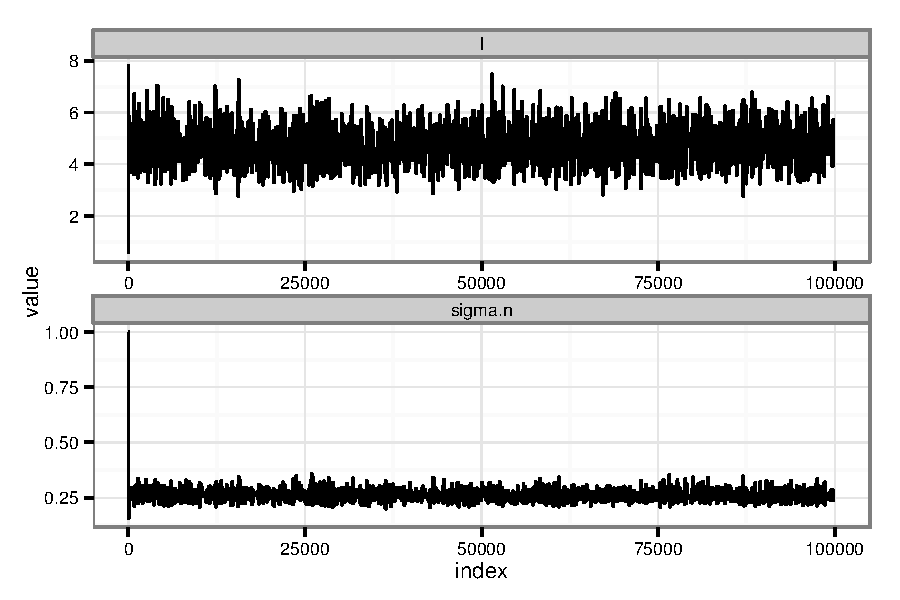
\includegraphics{gp_traces_densities1.pdf}
\caption{Traces of the GP hyper-parameters (after transforming back from
log space)}
\end{figure}

\begin{figure}[htbp]
\centering
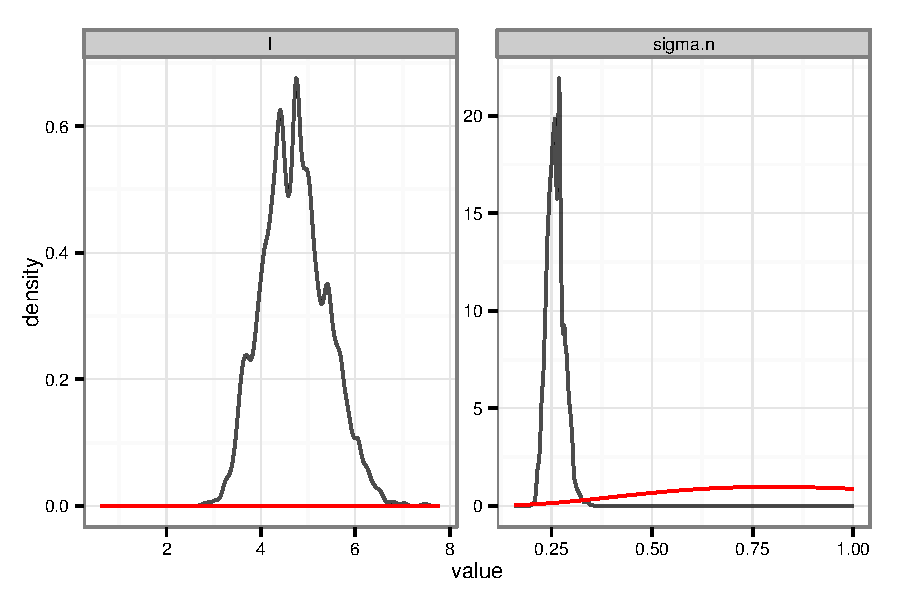
\includegraphics{gp_traces_densities2.pdf}
\caption{Posterior densities of the GP hyper-parameters (after
transforming back from log space). Prior distribution over the interval
sampled shown as red curves.}
\end{figure}

\begin{figure}[htbp]
\centering
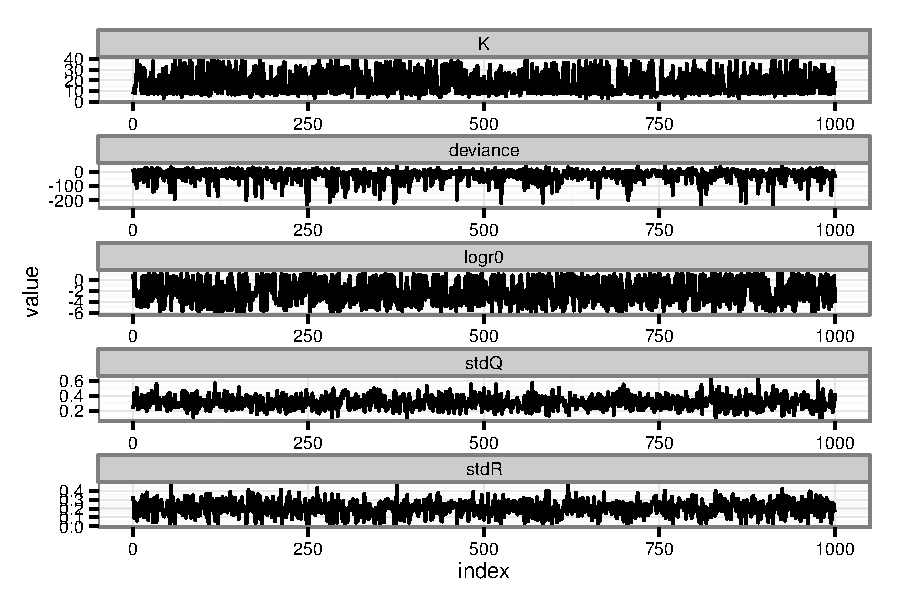
\includegraphics{ricker_traces.pdf}
\caption{Traces of the Ricker parameters}
\end{figure}

\begin{figure}[htbp]
\centering
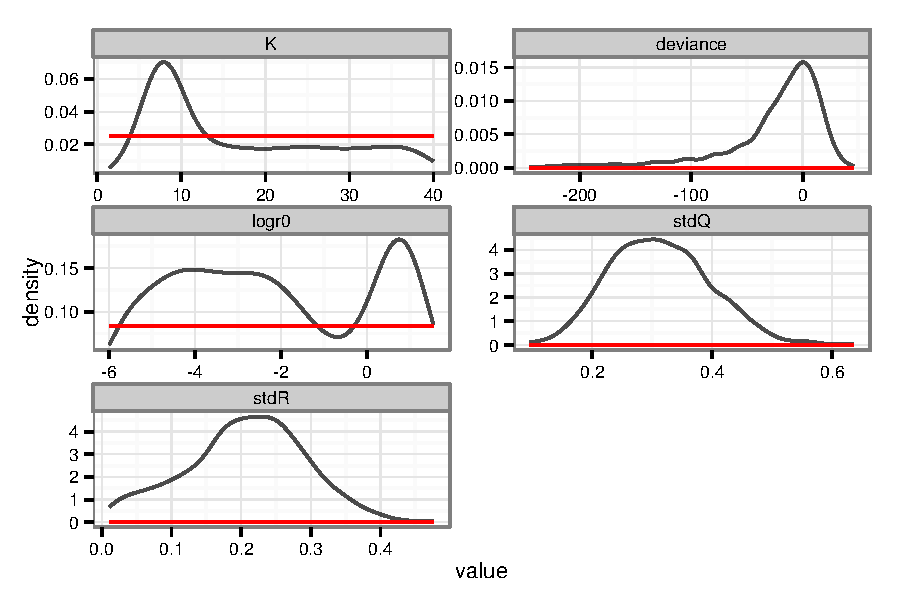
\includegraphics{ricker_posteriors.pdf}
\caption{Posterior densities of the Ricker parameter estimates. Prior
distributions over the interval sampled shown as red curves. Note the
bimodal estimate of $\log(r)$ which leads to the poor fit in Figure 1}
\end{figure}

\begin{figure}[htbp]
\centering
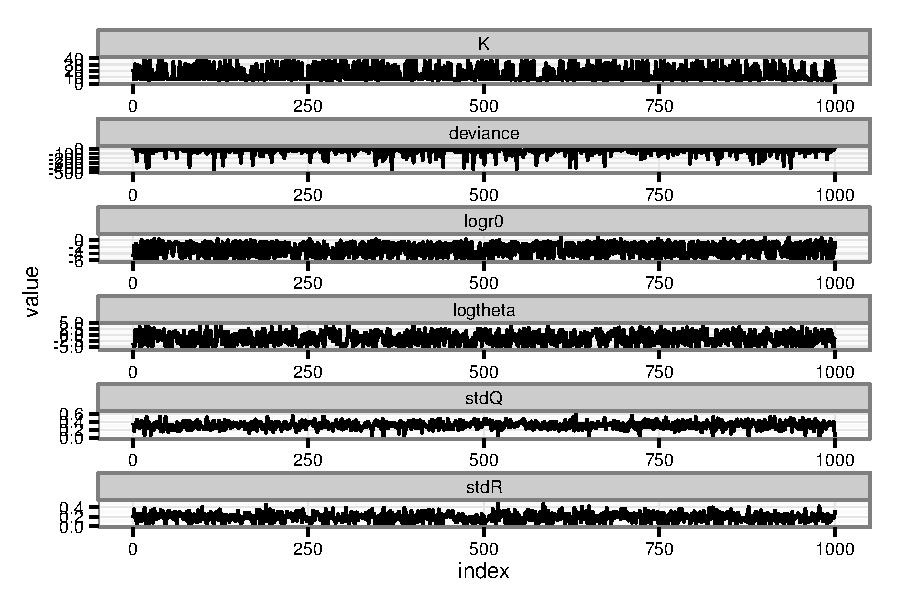
\includegraphics{parametric_bayes_traces.pdf}
\caption{Traces of the structurally accurate Allen model parameters}
\end{figure}

\begin{figure}[htbp]
\centering
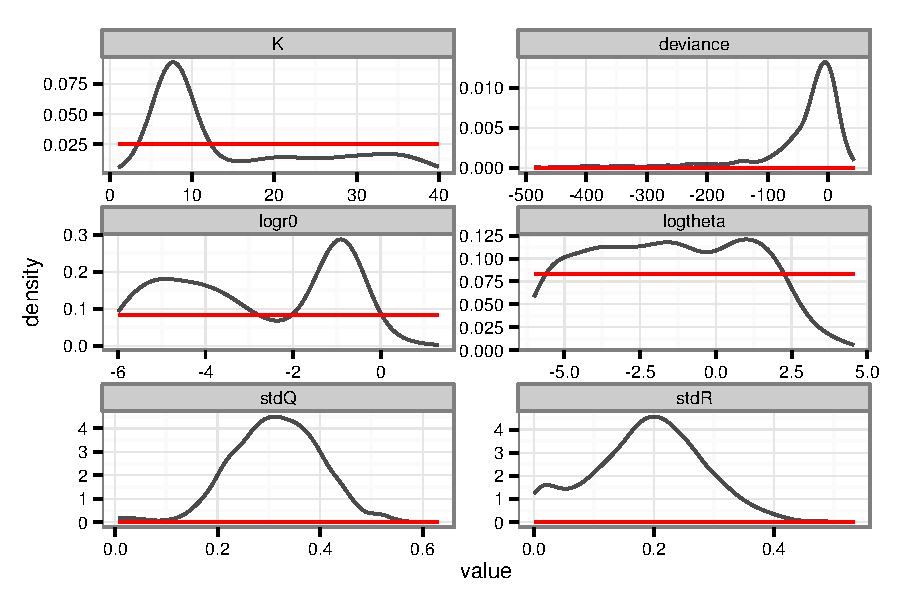
\includegraphics{parametric_bayes_posteriors.pdf}
\caption{Posterior densities for the parameters of the Allen model.
Prior distributions over the interval sampled shown as red curves.}
\end{figure}

\end{document}


